\documentclass[12pt, letterpaper] {article}

\parindent=5mm
\usepackage[spanish]{babel}

\usepackage{amssymb}
\usepackage{amsmath} 
\usepackage{amsfonts}

\usepackage[numbers,sort&compress]{natbib}
\usepackage{graphicx}

\usepackage{url}
\usepackage{hyperref}

\usepackage[top=25mm, bottom=20mm, left=1.5cm, right=1.5cm]{geometry}
\setlength{\parskip}{2mm}
\setlength{\parindent}{1pt}

\usepackage{listings}

\usepackage{float}

\usepackage[utf8]{inputenc}
\usepackage{graphicx} 
\usepackage{subfigure} 

\usepackage{color}
\usepackage{multirow}

\definecolor{dkgreen}{rgb}{0,0.6,0}
\definecolor{gray}{rgb}{0.5,0.5,0.5}
\definecolor{mauve}{rgb}{0.58,0,0.82}

\usepackage{color}
\usepackage{listings}
\lstset{ %
  language=R,                     % the language of the code
  basicstyle=\footnotesize,       % the size of the fonts that are used for the code
  numbers=left,                   % where to put the line-numbers
  numberstyle=\tiny\color{gray},  % the style that is used for the line-numbers
  stepnumber=1,                   % the step between two line-numbers. If it's 1, each line
                                  % will be numbered
  numbersep=5pt,                  % how far the line-numbers are from the code
  backgroundcolor=\color{white},  % choose the background color. You must add \usepackage{color}
  showspaces=false,               % show spaces adding particular underscores
  showstringspaces=false,         % underline spaces within strings
  showtabs=false,                 % show tabs within strings adding particular underscores
  frame=single,                   % adds a frame around the code
  rulecolor=\color{black},        % if not set, the frame-color may be changed on line-breaks within not-black text (e.g. commens (green here))
  tabsize=2,                      % sets default tabsize to 2 spaces
  captionpos=b,                   % sets the caption-position to bottom
  breaklines=true,                % sets automatic line breaking
  breakatwhitespace=false,        % sets if automatic breaks should only happen at whitespace
  title=\lstname,                 % show the filename of files included with \lstinputlisting;
                                  % also try caption instead of title
  keywordstyle=\color{blue},      % keyword style
  commentstyle=\color{dkgreen},   % comment style
  stringstyle=\color{mauve},      % string literal style
  escapeinside={\%*}{*)},         % if you want to add a comment within your code
  morekeywords={*,...}            % if you want to add more keywords to the set
} 
\usepackage{booktabs}
\usepackage[table,xcdraw]{xcolor}
\usepackage{epstopdf}



\author{Ricardo Rosas Macías}

\title{Práctica 6: Sistema multiagente}

\date{\today}

\begin{document}

\maketitle


\section{Introducción}
Un sistema multiagente es un método en donde los agentes interactúan los unos con los otros con ayuda de la inteligencia artificial, de tal modo que coordinan su comportamiento para llevar acabo una tarea de forma automática o resolver un problema complejo rápidamente.

 \section{Objetivo}
En términos generales,  se realizó cambios en el código de modo que permite vacunar a los agentes desde el inicio del experimento. Asimismo se cuantificó el porcentaje máximo de infectados en la ejecución del código.
 
 \subsection{Descripción}
 
Lo que se debe hacer es \cite{elisawebSMA}:
\begin{quotation}
 ``Vacunar con probabilidad $pv$ a los agentes al momento de crearlos de tal forma que están desde el inicio en el estado $R$ y ya no podrán contagiarse ni propagar la infección. Estudia el efecto estadístico del valor de $p_v$ en (de cero a uno en pasos de 0.1) el porcentaje máximo de infectados durante la simulación.''
\end{quotation}

\section{Resultados y conclusiones}

Para realizar acabo el experimento se tomaron los valores predeterminados del código del sitio web \cite{elisawebSMA}, como se muestra en la lista siguiente. 

\begin{lstlisting}[language=R]
l <- 1.5     
n <- 50      
pi <- 0.05 
pr <- 0.02 
v <- l / 30
r <- 0.1 
tmax <- 100 
\end{lstlisting}

Con ayuda de la paquetería \textit{listings} se colocaron las líneas de código modificado\cite{EMP6}. Asimismo se tomo las ponderaciones para la variación del experimento de 50 agentes en 30 repeticiones para la ejecución. En el cual los agentes se posicionaron de manera aleatoria en un rectángulo de medidas $L \times L$ en el cual todos sus extremos crean un continuo; como si fuese un toroide. Adicionalmente se programo para que el experimento se ejecutara con los agentes vacunados,  como se muestra en el inicio del código

\begin{lstlisting}[language=R]
pV <- c(0, 1, 0.1)
IMax <- c()
for(pv in pV) { 
  for(rep in 1:30) {
    agentes <- data.frame(x = double(), y = double(), dx = double(), dy = double(), estado  = character())
    for (i in 1:n) {
      e <- "S"
      if(runif(1) < pv) {
        e <- "R"
      } else {
        if (runif(1) < pi) {
          e <- "I"
        }
      }
      levels(agentes$estado) <- c("S", "I", "R")
      agentes <- rbind(agentes, data.frame(x = runif(1, 0, l), y = runif(1, 0, l), dx = runif(1, -v, v), 
               dy = runif(1, -v, v), estado = e))
    }
\end{lstlisting}

Por otra parte se ejecutó este código para obtener el efecto estadístico, de modo que se obtengan los datos, para posteriormente ser gráficados.

\begin{lstlisting}[language=R]
IMax <- c(IMax, max(epidemia))
  }
}
Vacu <- data.frame(Probvac = seq(pV, 30), Imaxi = (IMax/n)*100)
\end{lstlisting}

La ejecución del experimento mostró los resultados del análisis estadístico, que fue realizado mediante la prueba \textit{Kruskal-Wallis}, el cual evidencia que los datos tienen diferencias entre medianas estadísticamente significativas; debido a nivel de significación en donde el valor de $p$  es menor, como se muestra en el cuadro \ref{PKWE}.


\begin{table}[H]
\caption{Resultados de prueba Kruskal Wallis}
\label{PKWE}
\centering\begin{tabular}{|c|c|c|}
\hline
\rowcolor[HTML]{DAE8FC} 
{\color[HTML]{333333} Chi-squared} & df & p-value   \\ \hline
\rowcolor[HTML]{EFEFEF} 
{\color[HTML]{333333} 62.453}                     & 10 & 1.241e-09 \\ \hline
\end{tabular}
\end{table}


Por último, en la figura \ref{Ees} podemos apreciar que en cuanto más probabilidad de vacunados de 0 -- 1 en pasos de 0.1 el experimento tendrá un mejor control en el máximo de infección de los agentes. Además se puede apreciar una distribución uniforme y decreciente en los datos de la epidemia, como se muestra en la figura \ref{Ees} . 

\begin{figure}[H]
\centering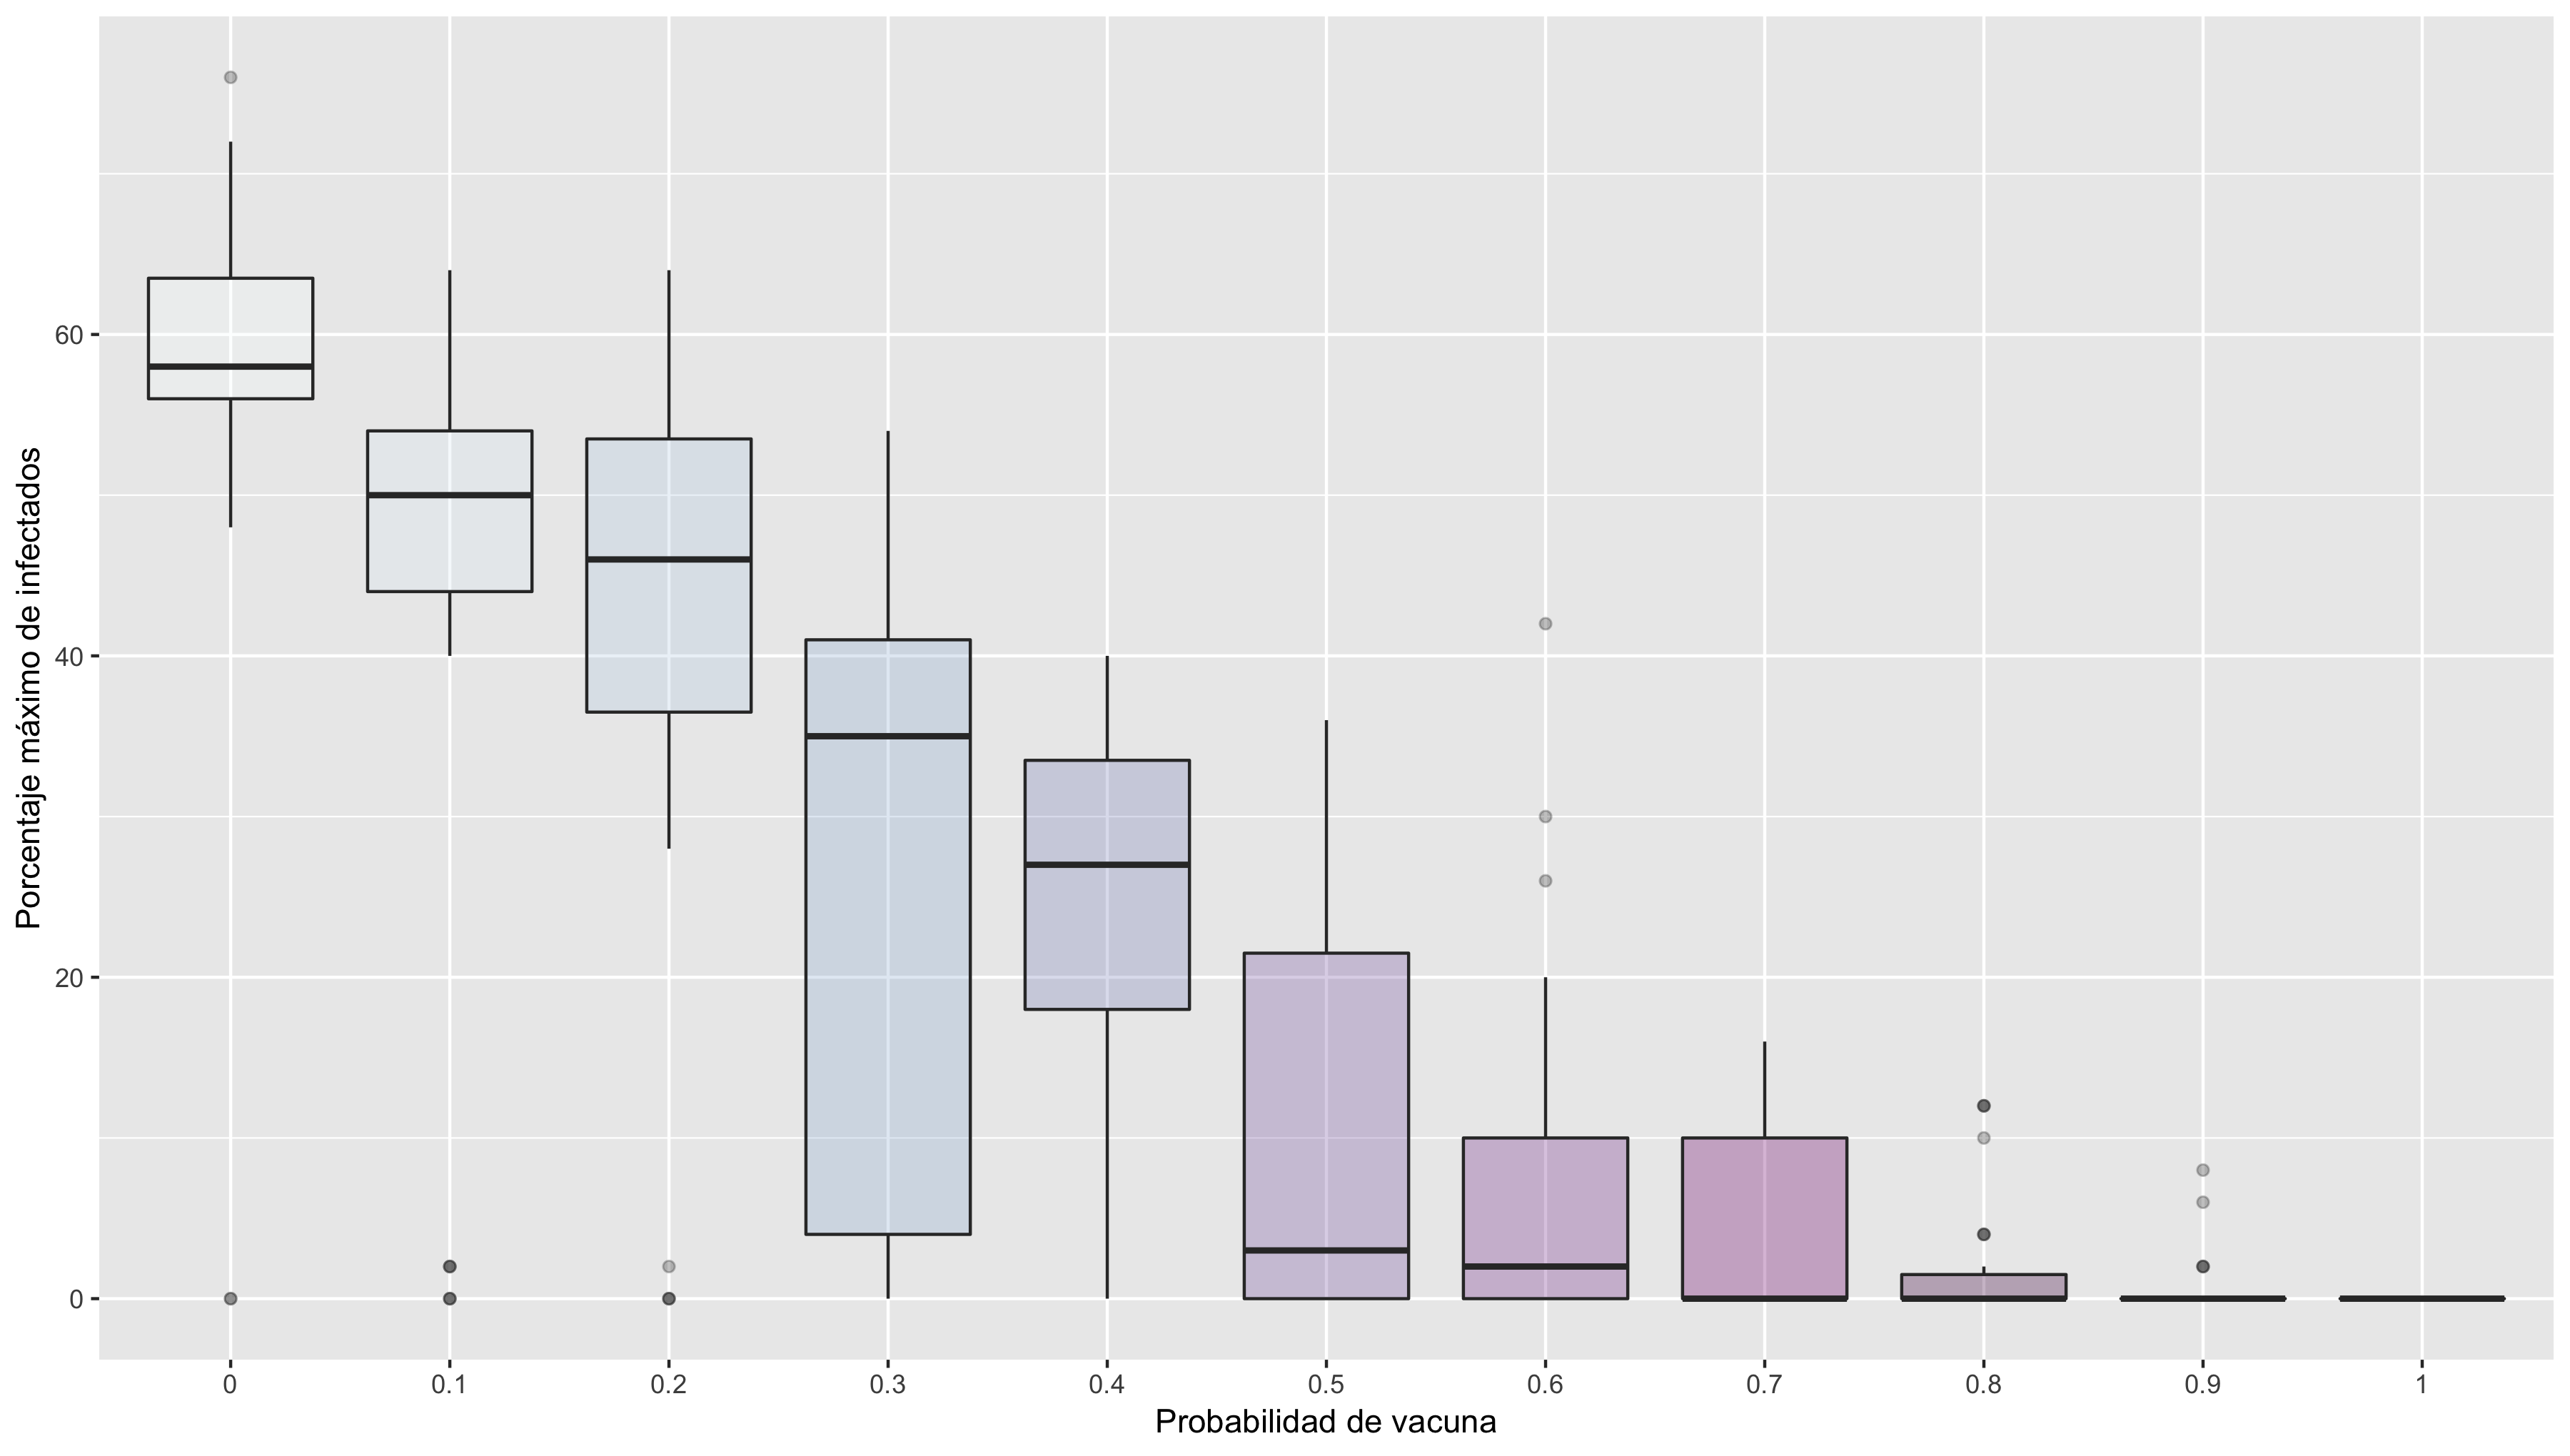
\includegraphics[width=150mm]{Avac.png}
\caption{Efecto estadístico}
\label{Ees}
\end{figure}


\bibliographystyle{plainnat}

\bibliography{BHWP6}

\end{document} 